\documentclass[conference]{IEEEtran}
\IEEEoverridecommandlockouts
% The preceding line is only needed to identify funding in the first footnote. If that is unneeded, please comment it out.
\usepackage{cite}
\usepackage{amsmath,amssymb,amsfonts}
\usepackage{algorithmic}
\usepackage{graphicx}
\usepackage{textcomp}
\usepackage{xcolor}
\def\BibTeX{{\rm B\kern-.05em{\sc i\kern-.025em b}\kern-.08em
    T\kern-.1667em\lower.7ex\hbox{E}\kern-.125emX}}
\begin{document}

\title{DRAFT: Reverse Image Search Documentation\\{\footnotesize May 1, 2022}}

\author{\IEEEauthorblockN{Jen McIntosh}
\IEEEauthorblockA{\textit{Brooklyn, NY \\
jgm9366@nyu.edu}}
\and
\IEEEauthorblockN{Shlok Goswami}
\IEEEauthorblockA{\textit{Brooklyn, NY \\
sg6862@nyu.edu}}
\and
\IEEEauthorblockN{
Ian Gray}
\IEEEauthorblockA{\textit{Brooklyn, NY \\
iwg210@nyu.edu}}
}

\maketitle

\begin{abstract}
Reverse-Image search is a popular service offered by a number of web search engines and media websites. The challenge that such a search presents primarily lies in the search's ability to accurately identify the contents of the image, and then match its features to those in an already existing database. It therefore becomes paramount to adapt a robust learning model which can accurately identify images, and to decide whether such an algorithm should concern itself more with subject identification or generalized (image-wide) feature matching. We first chose to implement our reverse-image search using a pretrained model ResNet50 and a $KNN$ algorithm. Improvements were then made introducing a deeper ResNet model and additional optimizers for the sake of fine tuning parameters. For these techniques our team makes made use of Tensorflow, Keras, and Sklearn libraries in Python. Reverse-image searches eventually have applications beyond simple online queries, and may be implemented wherever image recognition and extrapolation is needed.
\end{abstract}

\begin{IEEEkeywords}
CNN, sklearn, KNN, classifier, image search
\end{IEEEkeywords}

\section{Introduction}

The purpose of this project is to implement a system that can find faces within a dataset of images and videos, which later has applications in reverse-image searching. The system that we designed will search within a given dataset for a specific person of interest (POI) within the queried image. This sort of search is similar to pair matching or face verification. We begin by establishing a baseline model, which is tested on 10 query images from the Labeled Faces in the Wild (LFW) dataset. We then attempt to improve upon the baseline such that our reverse-image search returns more images, which based on features appear to be similar to the queried images.

\section{Dataset}

The pre-trained model implemented in ResNet50 is trained on ImageNet, and we begin our reverse-image search by first passing the Labeled Faces in the Wild (LFW) dataset through the search. The search result will return images from the LFW dataset that are most similar to the novel input image.

The ImageNet dataset consists of millions of pictures using a WorldNet hierarchy for data labels. It does not consist of solely human faces, as the LFW dataset does. Notably, roughly one fifth images within the ImageNet dataset include multiple objects, which has been shown by MIT researchers to lead to a 10\% drop in model accuracy\textsuperscript{1}. This setback will be discussed in later sections of this paper.

The LFW data set contains more than 13,000 images of faces, labeled with the name of the person pictured\textsuperscript{2}. The data set consists of several images which depict the same person. This is useful for the purposes of evaluating this reverse image search on faces, as inputting a face with known duplicates should result in a collection of similar images which contain multiple images of the same person.

\section{Methods}

For the purposes of this project, we chose to subjectively evaluate the accuracy of our search. We do this because users may have two distinct (although similar) main objectives with implementing a reverse image search: to find more images of a person/object in an image or to find images that are merely visually similar to the input image. The two objectives are distinct because two images of the same person may appear to be very different (the person is tanner in one photo and has a different hairstyle, for instance). Additionally, two visually similar images (based upon coloring, lighting, and positioning in the image) may depict vastly different subjects. Therefore we chose to classify a reverse-image search as accurate if it is able to correctly return primarily visually similar images, and secondarily images depicting the person in the query image.

The models and algorithms used to implement our baseline reverse-image search and subsequent improvements are detailed in the sections below.

\subsection{Baseline}
To establish our baseline reverse-image search we implemented a pre-trained deep learning ResNet50 model with its top layer removed, and then implemented a nearest neighbor algorithm. The RestNet50 model is pre-trained on ImageNet, which is detailed in section III of this paper. The ResNet50 model converts images into just 2048 features, far fewer than other deep learning modules, which will expedite our search and nearest neighbor algorithm. Additionally, as the purpose of this model is to merely establish a baseline, the small number of features presents a potential area for (accuracy) improvement. We remove the top layer of ResNet50 so that the model returns convolved features rather than classification probabilities. We then fit our resulting feature vectors (consisting of 2048 features each) to one of Scikit Learns (Sklearn) nearest neighbor algorithms. For the purposes of establishing a baseline we chose the ball\_tree algorithm. 

To implement a reverse-image search on faces, we first pass the LFW dataset through the RestNet50 pre-trained model and fit the resulting feature vectors to the nearest neighbor algorithm as previously described. From there we take the image to be "reverse searched," which is an image not present in the training dataset (hopefully), and again create the 2048 feature vector using ResNet50 and find its nearest neighbors from the LFW dataset. With the nearest neighbors' indices we are able to then return the most similar images from the LFW dataset.

\subsubsection{ResNet50 Architecture}

ResNet is short for Residual Networks, and it was one of the first neural networks to allow training of 150+ layered deep neural networks without the problem of vanishing gradients. Vanishing gradients often arise as network depth increases - as a gradient is back-propagated over several layers the repeated multiplication makes the gradient negligible. This phenomenon causes saturated, and eventually degrading, performance of the neural network. 

ResNet tackles the problem of vanishing gradients through the use of skip connections. Equation 2 summarizes, in essence, what a skip connection entails. The skip connection adds the original input layer to the convolved layer post-convolution, therefore the layers (original and convolved) must be of the same size. This is achieved by either outputting a convolved layer which is of the same size as the input, or by passing the original layer through a separate convolution layer resulting in the same size as the target convolved layer. Skip connections are applied prior to ReLU activation. Skip connections are useful when dealing with vanishing gradients because they provide an alternate route for gradients AND they allow the model to learn an identity function. The identity function ensures that higher layers will not perform worse than lower layers.

The whole ResNet50 model consists of 5 stages, each with its own convolution and identity block. Each block has 3 convolution layers. Overall, the model has 23 million trainable parameters. The below figure illustrates the overall ResNet50 architecture along with the contents of the convolution and identity blocks.

\begin{figure}[h]
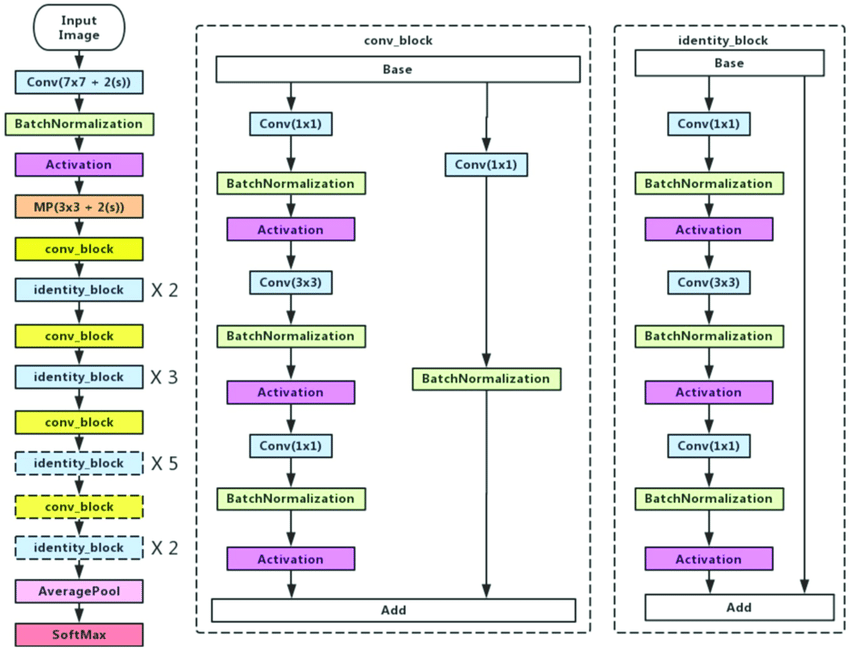
\includegraphics[width=7cm]{resnet50 arch.png}
\centering 
\caption{ResNet50 Architecture\textsuperscript{3}}
\label{fig:1}
\end{figure}

Note that in our model we do not include the final average pooling and soft max layers. These layers create an output of class probabilities, whereas without them the ResNet50 model outputs feature maps.

\subsubsection{$K$ Nearest Neighbors}
The $K$ Nearest Neighbors algorithm simply takes a new/input vector and finds the $k$ vectors within a stored train set which are "nearest" or "closest" to the input vector. It assigns the most frequent label amongst the $k$ neighbors to the new/input vector. Our KNN algorithm uses Euclidean distance as the metric to measure neighbor distance. Euclidean distance is defined as:

\begin{equation}
d_{ED}= \sqrt{ (x_1-y_1)^2 + (x_2-y_2)^2 + (x_3-y_3)^2 } \label{eq:1}
\end{equation}
Where $\textbf{x}=<x_1,x_2,x_3>$ and $\textbf{y}=<y_1,y_2,y_3>$ are vectors. This is also often called the L2 norm of $\textbf{x}-\textbf{y}$.

We first fit the results of the KNN algorithm run in the LFW dataset to the feature map produced by our model (2048 features), and use this to compare the new/input vector to the LFW dataset. Because of the large number of features, the KNN algorithm may be unable to accurately cluster similar features, and may be subject to overfitting, therefore we then reduced the size of our feature map to 1500 and used this to fit the KNN algorithm. 

\subsubsection{Baseline Results}
The below screenshots depict an input image and corresponding outputs, both before and after reducing the size of our feature map for KNN fitting. Note that this image is not one of our ten query images, and our reverse-image search is implemented to output 20 images. The output is scaled down for the purposes of this paper.

\begin{figure}[h]
    \centering
    \caption{Input Image for Establishing Baseline}
    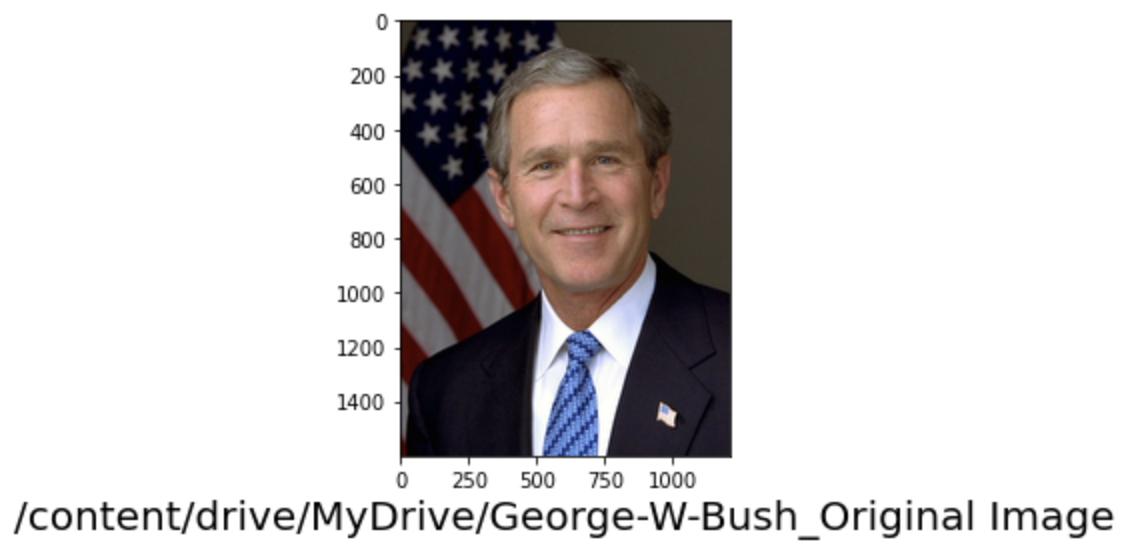
\includegraphics[width=7cm]{gwbush.png}
    \label{fig:2}

    \caption{Baseline Output Before Reducing FM Size}
    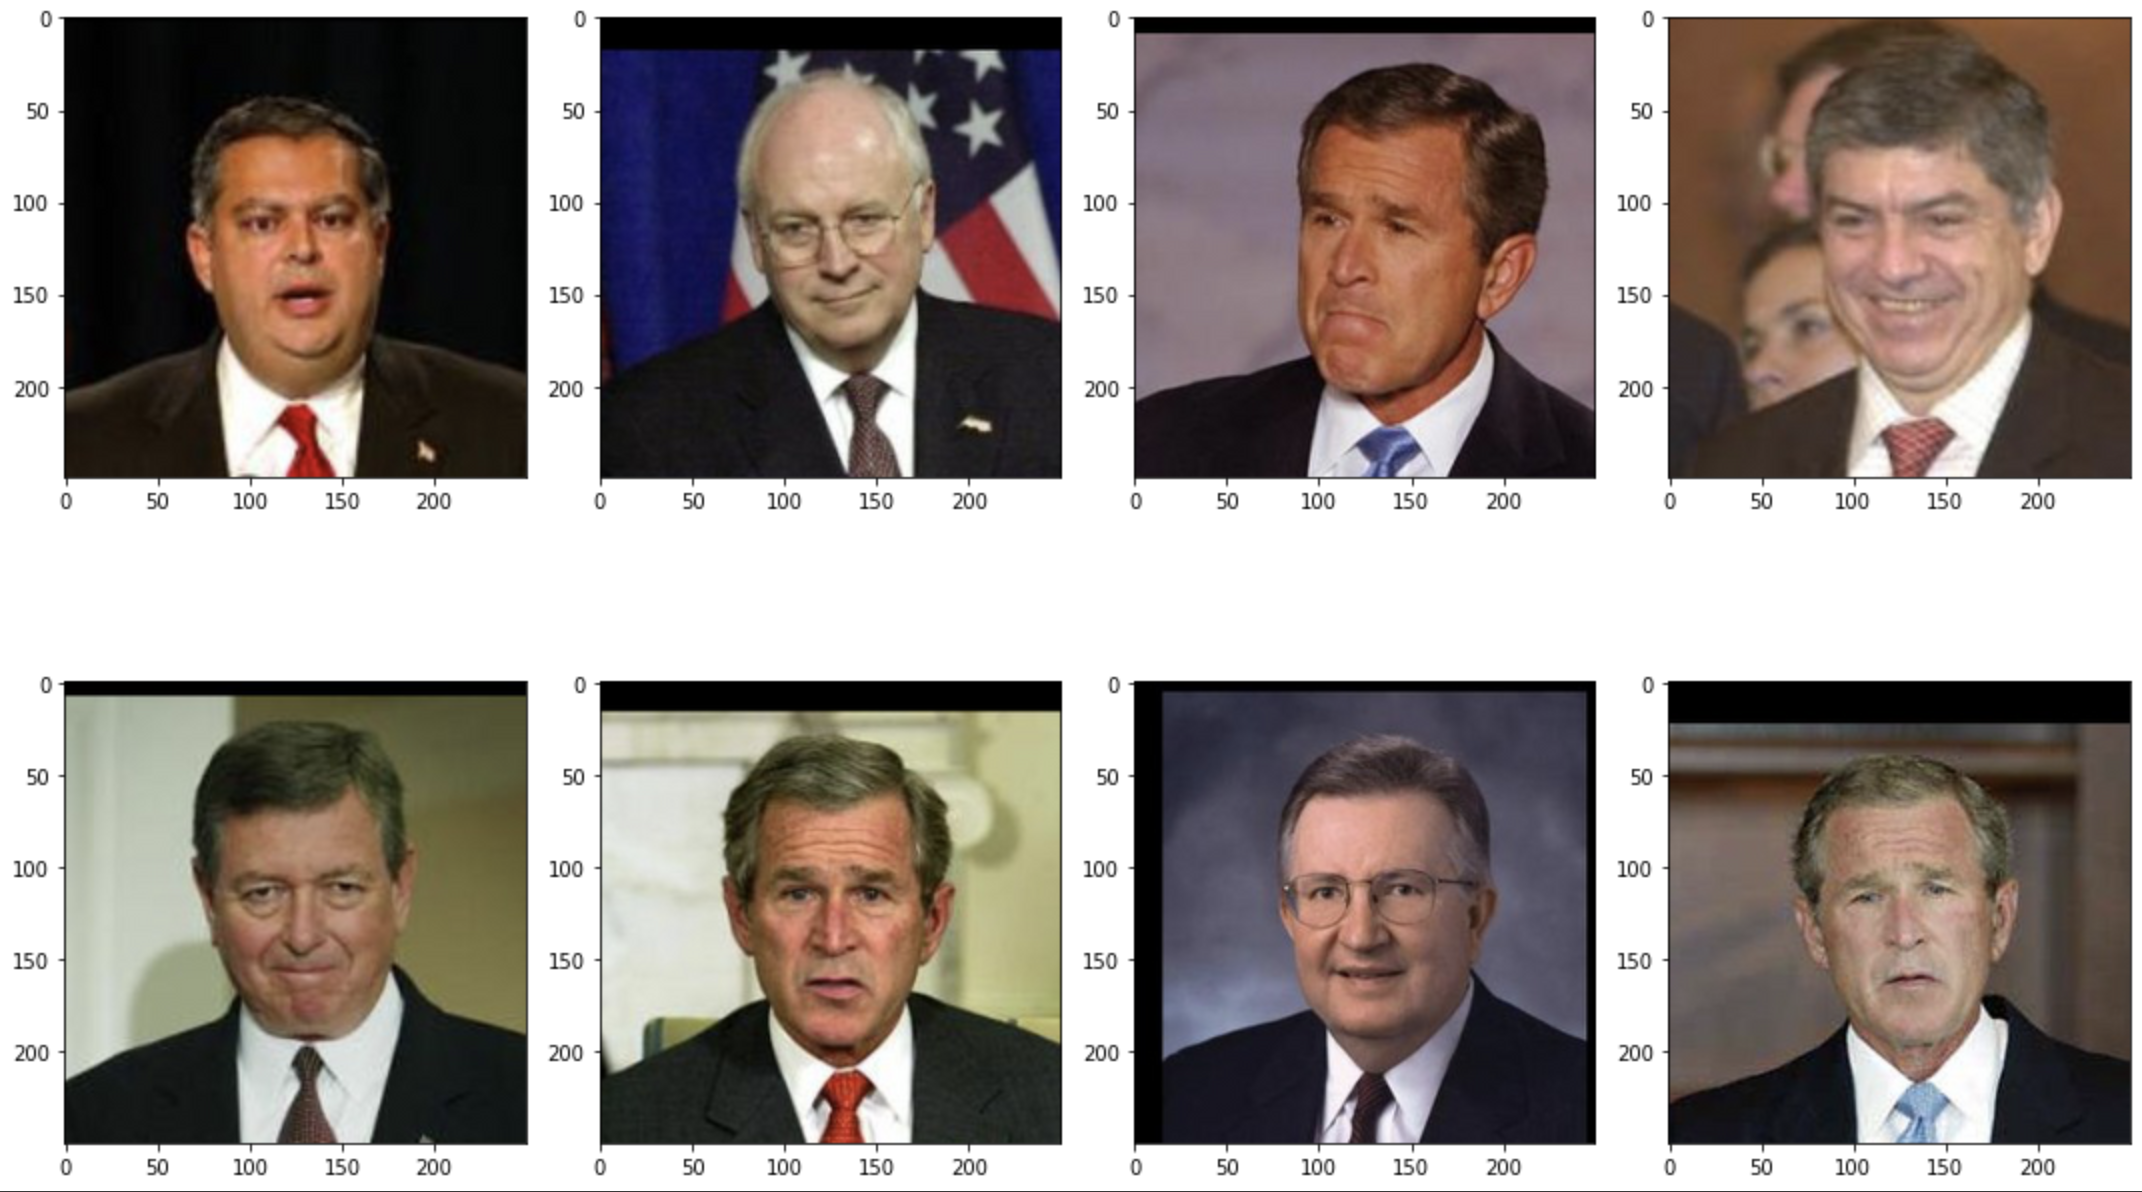
\includegraphics[width=7cm]{og_baseline.png}
    \label{fig:3}
    
    \caption{Baseline Output After Reducing FM Size}
    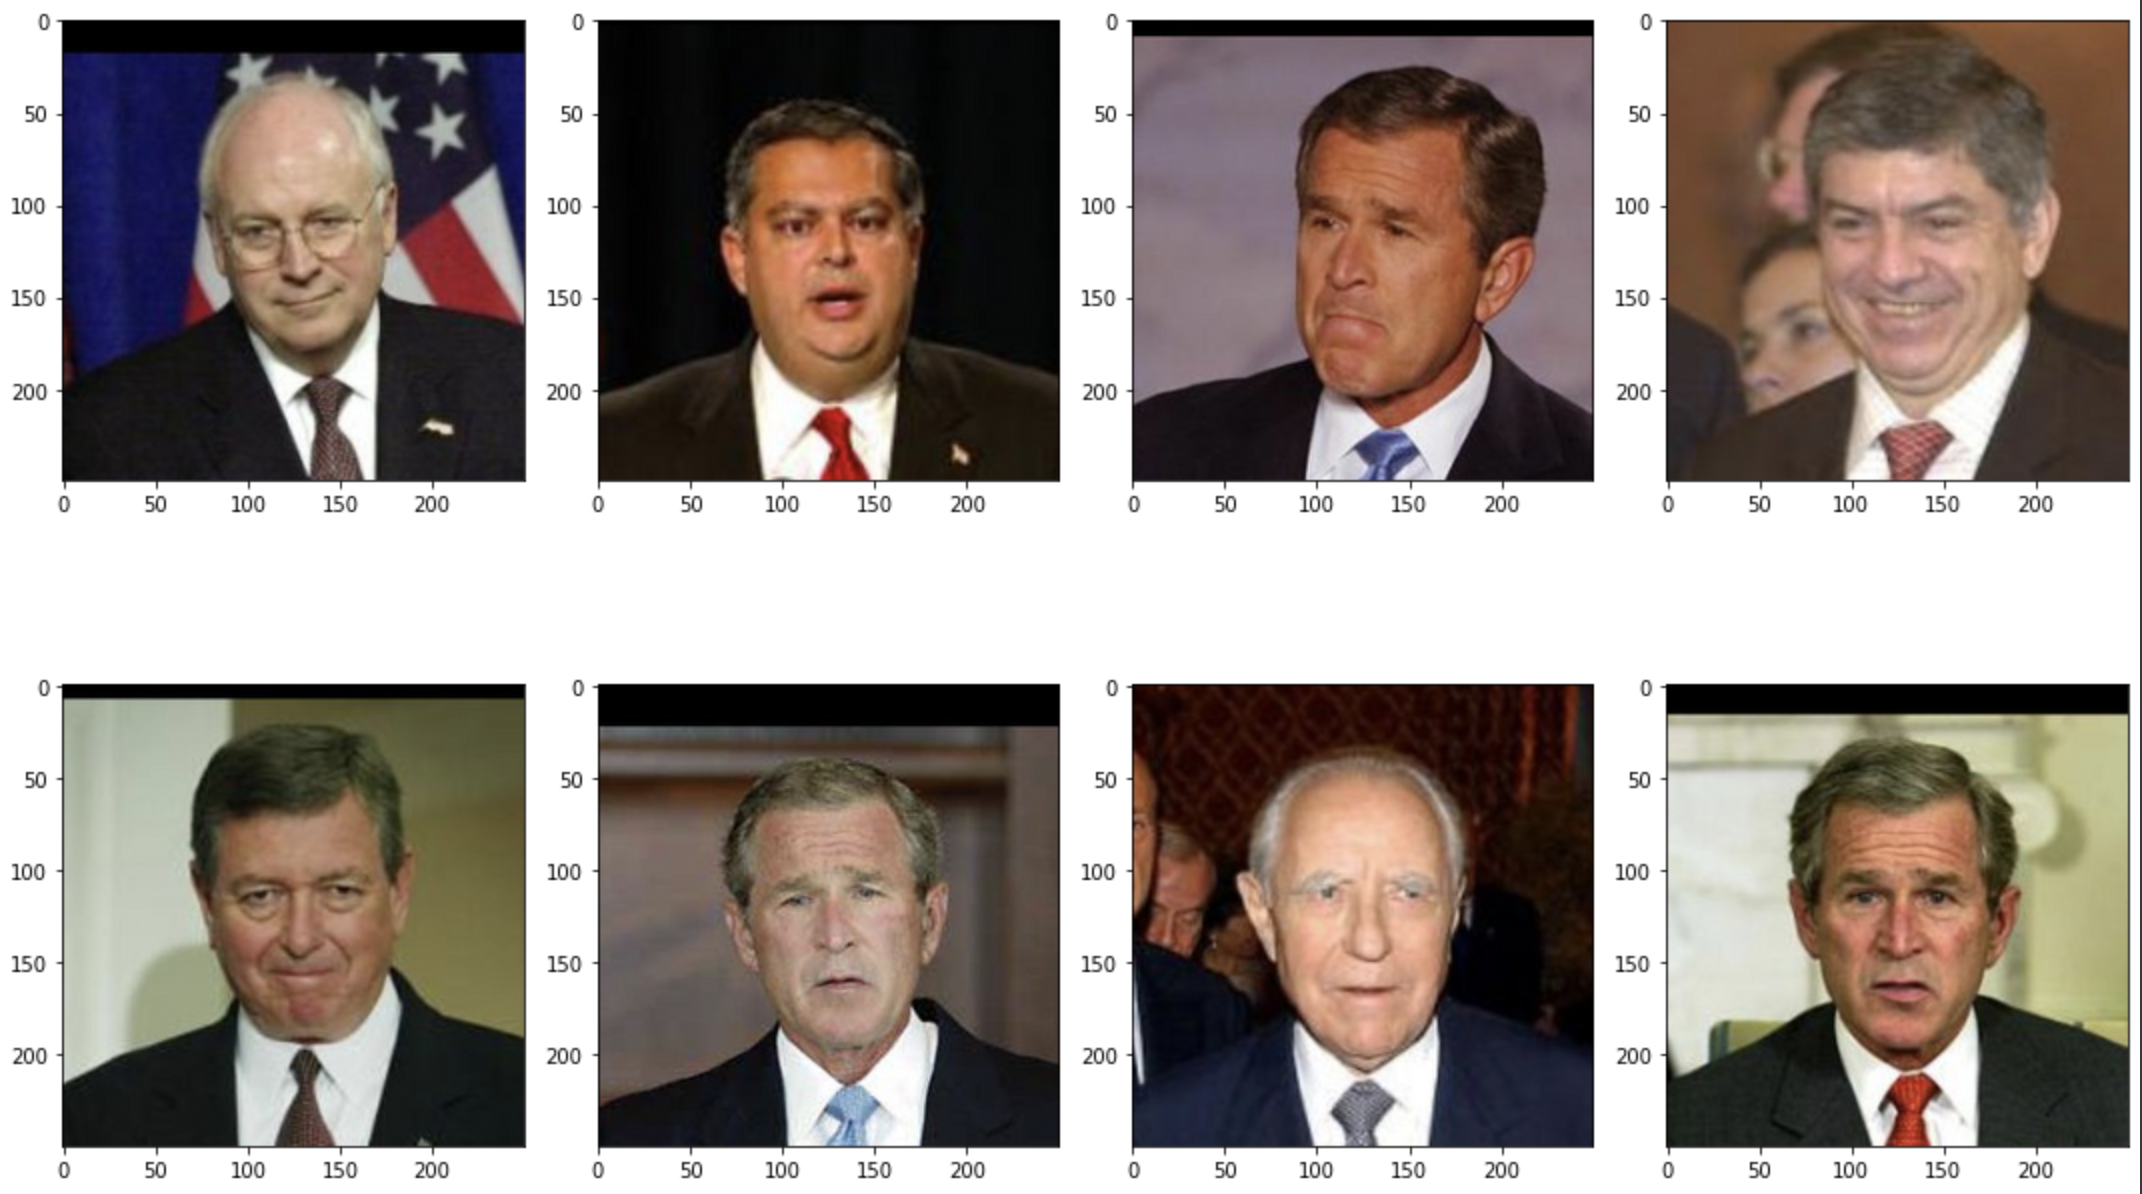
\includegraphics[width=7cm]{pca_baseline.png}
    \label{fig:4}
    \centering
\end{figure}

Interestingly enough, we noted that there was no noticeable improvement after reducing the size of our feature map, and with too many reductions ($<1000$ features) there was a degradation in search performance. This is something we address when we make improvements to this baseline.

\subsection{Improvements}

To improve upon our baseline we chose to implement the ResNet101 model, an Adamax optimimzer, and to decrease the batch size of our model from 64 to 16. We also chose to not constrain the number of features in our model's initial feature map output (2048 features). Our ResNet101 model is initialized similarly to the baseline ResNet50 model in that we again chose to remove the top layers and pre-train on the ImageNet dataset. The addition of the Adamax optimizer, an extension of Stochastic Gradient Descent, is to fine-tune our model's parameters. This optimizer, in addition to the decreased batch size, enabled our model to better fit its parameters. 

\subsubsection{ResNet101 Architecture}

ResNet101 is similar in architecture to the ResNet50 model, except that it has 101 layers rather than 50 (as the name suggests). It therefore also benefits from skip connections (sometimes called residual mapping) and therefore the increased depth does not force the gradients used in back-propagation to vanish. The below image is an overview of this model's architecture and how it compares to ResNet50 and ResNet34.\textsuperscript{7}

\begin{figure} [h]
    \centering
    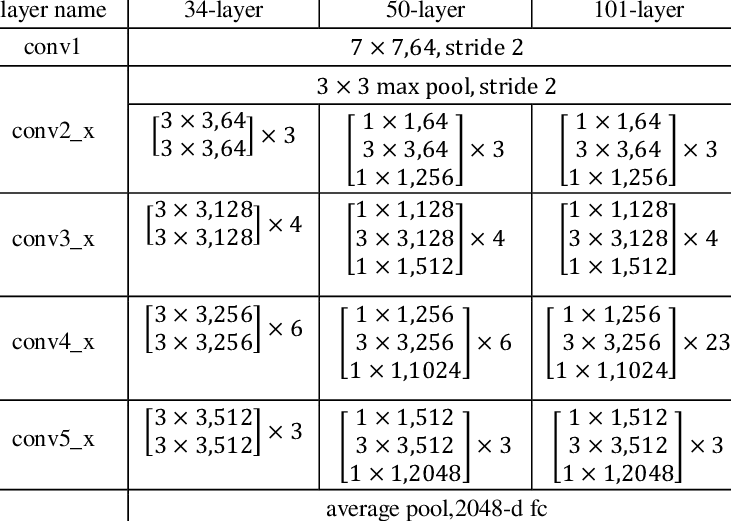
\includegraphics[width=7cm]{resnet compare.png}
    \caption{Comparing ResNet 34, 50, and 101}
    \label{fig:5}
\end{figure}

\begin{figure} [h]
    \centering
    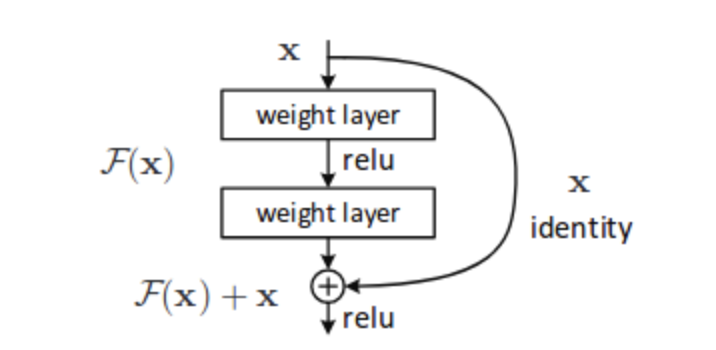
\includegraphics[width=7cm]{skip ex.png}
    \caption{A diagram illustrating skip connections/residual mapping}
    \label{fig:6}
\end{figure}


\subsubsection{Adamax Optimizer}

Adamax is an extension of Adam (Adaptive Movement Estimation) which generalizes Adam's approach to the infinite norm from the L2 norm that is traditionally used. Adam itself is is based on stochastic gradient descent, however it is unique in that it requires only first-order gradients and computes individual adaptive learning rates for each parameter in the function/model to be optimized. A thorough and concise overview of Adam is provided by Kingma et al.\textsuperscript{8} Adamax, with the addition of the infinite norm approach, is a stabler version of Adam which is more robust against noise. Adam and Adamax additionally make use of an $\epsilon$ for added stability.


\subsubsection{Improvement Results}
Altogether, these changes yielded results which contained more visually similar subjects, regardless of variation in background. We judge this to be an improvement upon the baseline because we received images which contained the same person as our input AND people who are visually similar to the person in our input image. The below is a screenshot of our results run with the same test image as above, this time with 20 output images.

\begin{figure}[h]
    \centering
    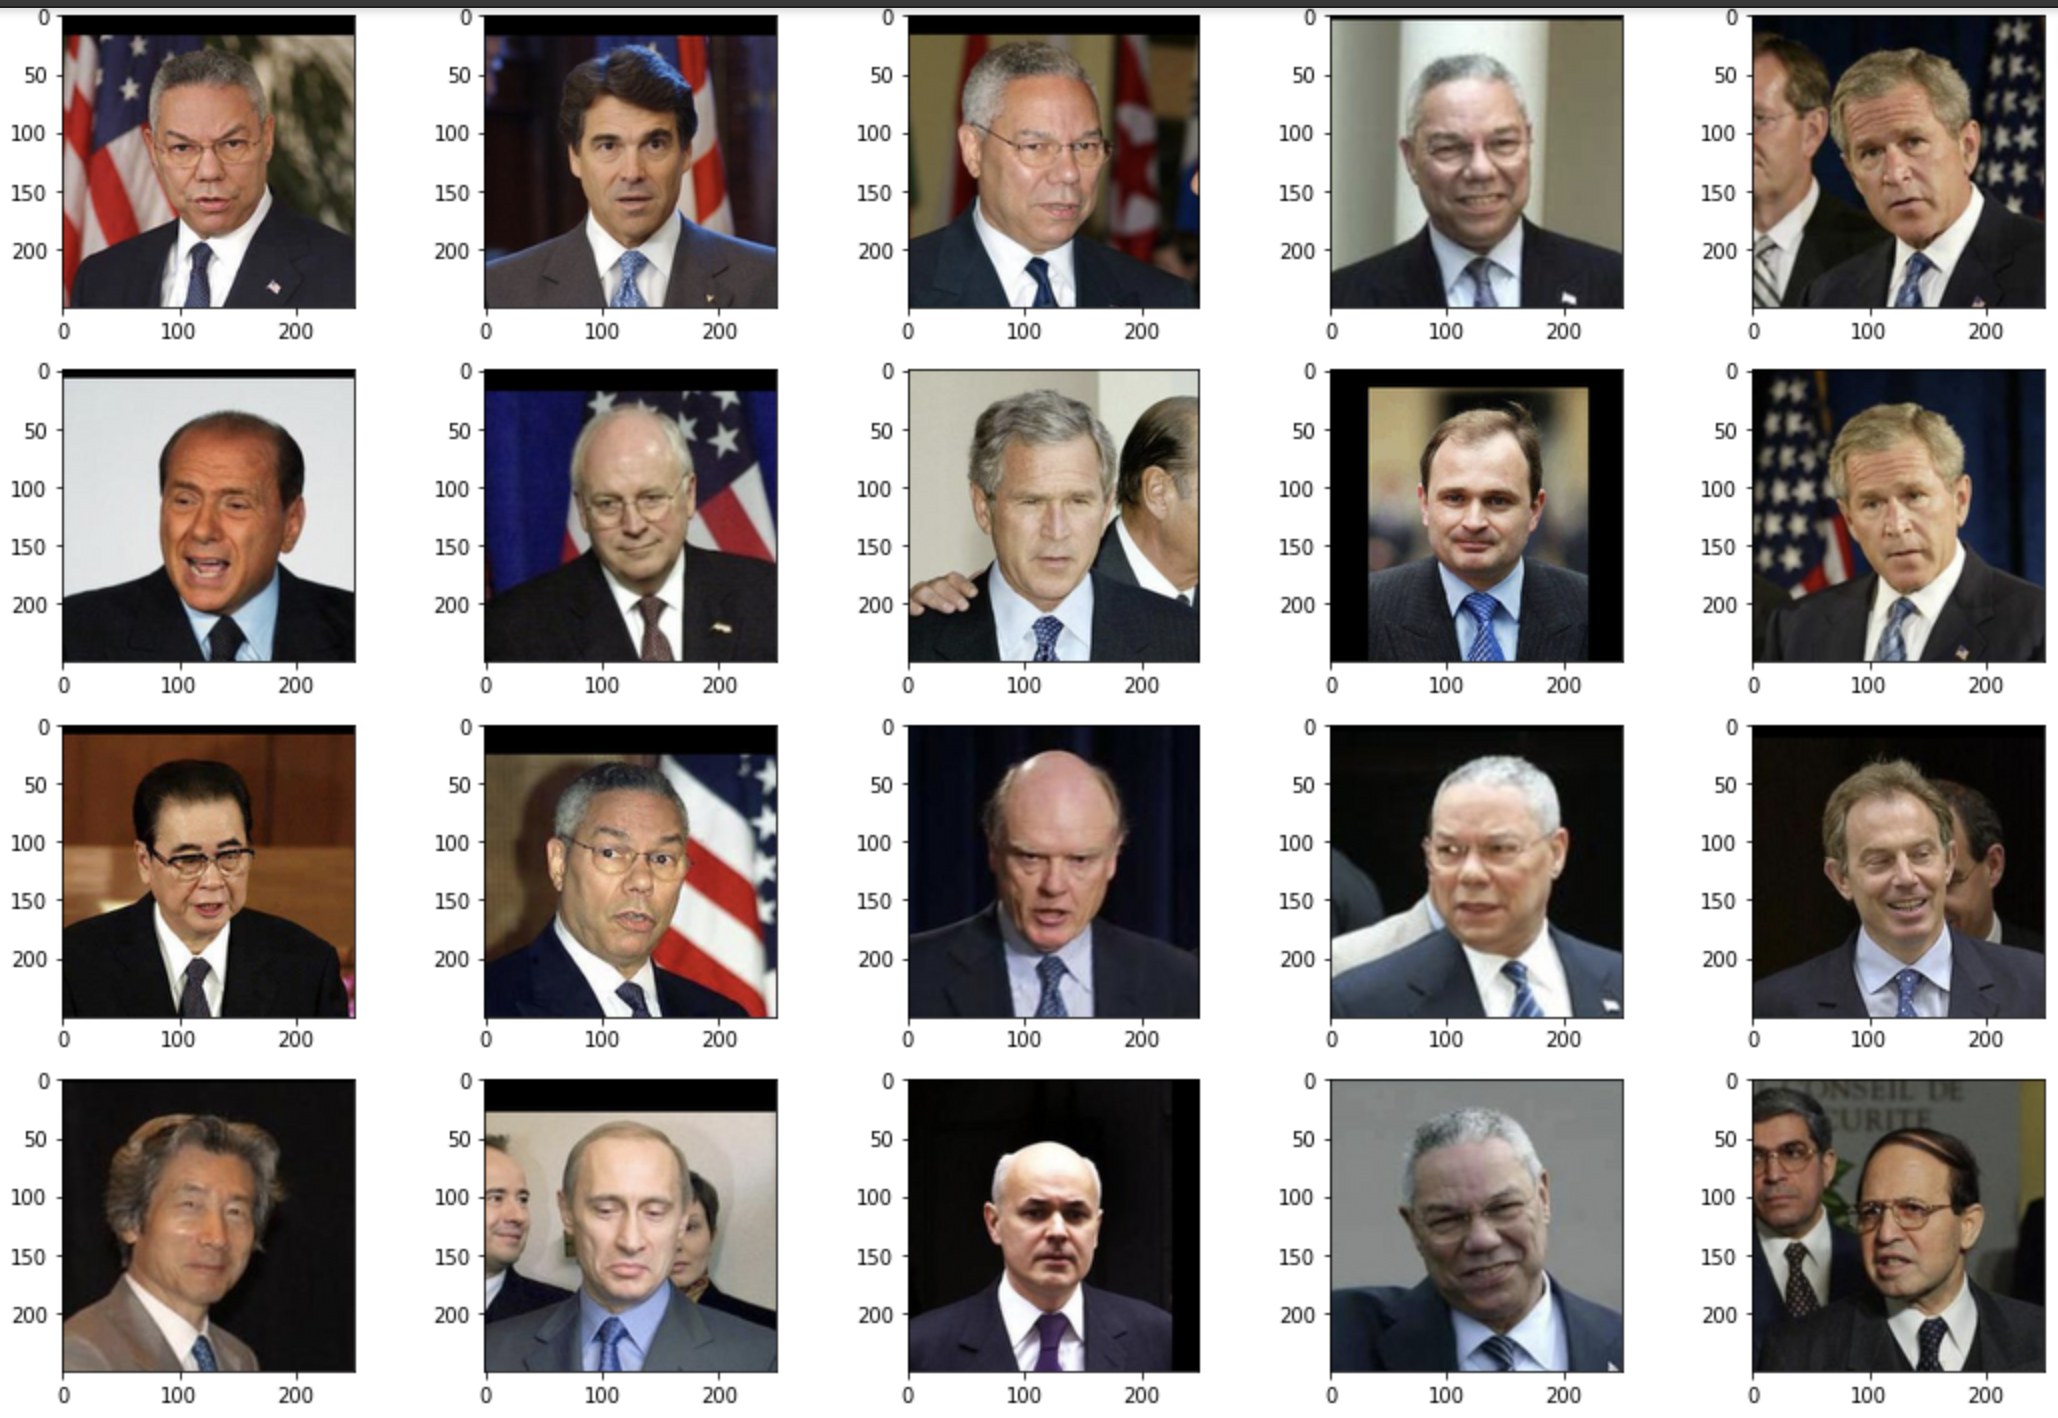
\includegraphics[width=7cm]{improvement.png}
    \caption{Output of query image on Reverse-Image search implemented with ResNet101, Adamax, and smaller batch size}
    \label{fig:7}
\end{figure}



\section{Equations}
Here will be some relevant math if it ends up being necessary.....

\begin{equation}
   X_o+X_c = Add[X_o,X_c] :
   \label{eq:2}
\end{equation}
$$
\begin{bmatrix}
x_{1,1}^o & ... & x_{n,1}^o\\
... & ... & ...\\
x_{1,n}^o & ... & x_{n,n}^o\\
\end{bmatrix}
+
\begin{bmatrix}
x_{1,1}^c & ... & x_{n,1}^c\\
... & ... & ...\\
x_{1,n}^c & ... & x_{n,n}^c\\
\end{bmatrix}
$$
$$
=
\begin{bmatrix}
x_{1,1}^o+x_{1,1}^c & ... & x_{n,1}^o+x_{n,1}^c\\
... & ... & ...\\
x_{1,n}^o+x_{1,n}^c & ... & x_{n,n}^o+x_{n,n}^c\\
\end{bmatrix}
$$





\section{Conclusion}


Some drawbacks to this model stemming from the LFW dataset:
\begin{itemize}
    \item Many groups are underrepresented by the LFW dataset, including babies, children, elderly people, and women.
    \item There are few instances of additional conditions such as low light, strong occlusion, and low resolution in the dataset.
    \item It is very difficult to extrapolate to N sized inputs.
    \item The dataset is not robust enough to create strong statistical conclusions about subgroups, and many minority ethnicities are either underrepresented or absent.
\end{itemize}

Additionally, both our baseline and improved image search seem to preference facial expression and clothing (particularly color) over generalized facial features. This is one significant area for improvement and future work, where ideal models would be those which are able to learn features given an array of expressions and extrapolate to other facial expressions made by the same person. 

Ideal models would also be those which are able to discern and then ignore clothing. They might also distinguish key features like eyes, nose, mouth and use feature maps drawn from this anatomy specifically as heavily weighted parameters, while other elements which are subject to variability (within individuals) like hair, skin tone, and fashion are afforded less weight.

Finally, an interesting avenue to explore would be how a model might make use of recursion on learned faces and use predicted facial expressions (i.e., a model is given multiple images of someone frowning and laughing and attempts to predict a feature map of the same person smiling) as an additional feature maps to fit in a $KNN$ algorithm.

\begin{thebibliography}{00}
\bibitem{b1} Johnson, K. "MIT researchers find 'systematic' shortcomings in ImageNet Data set." \textit{VentureBeat}. July 15, 2020.  https://venturebeat.com/2020/07/15/mit-researchers-find-systematic-shortcomings-in-imagenet-data-set 
\bibitem{b2} Gary B. Huang, Manu Ramesh, Tamara Berg, and Erik Learned-Miller.
"Labeled Faces in the Wild: A Database for Studying Face Recognition in Unconstrained Environments." \textit{University of Massachusetts, Amherst, Technical Report 07-49}, October, 2007.
\bibitem{b3} Ji, Qingge \& Huang, Jie \& He, Wenjie \& Sun, Yankui. (2019). "Optimized Deep Convolutional Neural Networks for Identification of Macular Diseases from Optical Coherence Tomography Images." \textit{Algorithms}: Vol 12. pg. 51. doi: 10.3390/a12030051. 
\bibitem{b4} Rosebrock, A. "Fine-tuning resnet with keras, tensorflow, and Deep Learning," \textit{PyImageSearch}. 2021, April 17.  https://pyimagesearch.com/2020/04/27/fine-tuning-resnet-with-keras-tensorflow-and-deep-learning/ 
\bibitem{b5} "Keras Documentation: Keras applications," \textit{Keras}. https://keras.io/api/applications/ 
\bibitem{b6} Bin Li, Dimas Lima. (2021). "Facial expression recognition via ResNet-50,"
\textit{International Journal of Cognitive Computing in Engineering}: Vol 2. pgs. 57-64.
ISSN 2666-3074. doi: 10.1016/j.ijcce.2021.02.002.
\bibitem{b7} Wu, Huiyan & Xin, Ming & Fang, Wen & Hu, Hai-Miao & Hu, Zihao.  "Multi-Level Feature Network With Multi-Loss for Person Re-Identification," \textit{IEEE Access}. pg. 1 2019 10.1109/ACCESS.2019.2927052.
\bibitem{b8} Kingma, Diederik P. and Ba, Jimmy. "Adam: A Method for Stochastic Optimization," \textit{3rd International Conference for Learning Representations}, 2015. 
https://doi.org/10.48550/arXiv.1412.6980

\end{thebibliography}
\vspace{12pt}

\end{document}
